\documentclass[12pt]{article}
\usepackage{amsmath}
\usepackage{amsfonts}
\usepackage{hyperref}
\usepackage{fullpage}
\usepackage{booktabs}
\usepackage{xspace}
\usepackage{longtable}
\usepackage[toc,page]{appendix}

% Much nicer visual links
\hypersetup{
    colorlinks=true,
    linkcolor={red!50!black},
    citecolor={blue!50!black},
    urlcolor={blue!80!black}
}

% To do note packages. Remove when complete.
\usepackage{todonotes}
\newcommand{\note}[1]{\todo[inline]{#1}}
\newcommand{\needref}{\mbox{({\color{blue}\rule{.3cm}{.3cm}} REF)\xspace}}

% Counters for number of edits made to OEIS
\newcommand{\OEISedits}{XXX\xspace}
\newcommand{\OEISprimary}{XXX\xspace}

\newcommand{\OEIS}[1]
{\href{https://oeis.org/#1}{\texttt{#1}}}

% Text shortcuts
\newcommand{\SEQ}{\mathcal{S}}
\newcommand{\CLASS}{\mathcal{C}}
\newcommand{\SIMPLECLASS}{\mathcal{C}_\text{simple}}
\newcommand{\ie}[0]{i.e.\ }

\setlength{\parindent}{.35cm}

\begin{document}

\title{Integer sequence discovery from small graphs}
\author{Travis Hoppe and Anna Petrone}
\date{\today}
\maketitle

\begin{abstract}
We exhaustively enumerate all simple, connected graphs of a finite order and compute a selection of invariants over this set.
Integer sequences were constructed from these invariants and checked against the Online Encyclopedia of Integer Sequences (OEIS).
\OEISprimary new sequences were added and \OEISedits sequences were appended or corrected.
From the graph database we are able to programmatically suggest relationships among the invariants.
We show that we can readily visualize any sequence of graphs with a given criteria.
The code has been released as an open-source framework for others to add additional invariants not considered in this work.
\end{abstract}

\section{Introduction}

\note{Add introduction, detail why project is important}
\note{mention it is good for benchmarks, cite Santo paper. Cite other publicly available databases such as those in the House of Graphs intro, mention how this is more exhaustive and give DOI for project.}

The Online Encyclopedia of Integer Sequences (OEIS) was created by Neil Sloane in 1964.
As a graduate student, Sloane began collecting integer sequences while studying combinatorial problems.
Since then, the database has grown to over 250,000 sequences and is highly cited, with over 3,000 citations to date\cite{sloane2003line}.
The sequences are of general interest, spanning topics such as number theory, combinatorics, and graph theory.
A given sequence may contain any number of terms, ranging from at least four up to as many as 500,000 in the cases where the sequence admits a readily computable expression.
Collecting and storing integer sequences in one place allows a researcher, who perhaps comes across the first few values of an unknown sequence, to be able to quickly look up subsequent values. 
The OEIS not only provides the numerical values but seeks to function as a true encyclopedia, with cross references to related sequences, references to other literature, and formulas when known.
One of the primary goals of this project was to systematically expand the sequences involving graph invariants known to the OEIS database.
Through our exhaustive enumeration of all small graphs, we were able to submit \OEISprimary new sequences to the OEIS and extend \OEISedits existing sequences.

A graph invariant is any property that is preserved under isomorphism. 
Invariants can be simple binary properties (planarity), integers (automorphism group size), polynomials (chromatic or Tutte polynomials), rationals (fractional chromatic numbers), complex numbers (adjacency spectra), sets (dominion sets) or even graphs themselves (subgraph and minor matching). 
We are primarily concerned with the sequences produced by graph invariants, \ie the combinatorial problem of how many graphs of a given class satisfy a particular criteria.
Let a graph be defined as the pair $G = (V,E)$, where $V$ is a set of vertices and $E$ a set of edges. 
Define $\CLASS$ as a class which forms an isomorphically distinct set of graphs that satisfy a specified criteria.
Group the graphs into non-overlapping subsets such that
\begin{equation}
\CLASS = \CLASS_1 \cup \CLASS_2 \cup \CLASS_3 \cup \ldots
\end{equation}
where $\CLASS_n$ contains only graphs of order $n$.
From here, define an ordered sequence of subsets of the graph class
%
\begin{align}
\SEQ(f, \CLASS) 
&= f(\CLASS_1), f(\CLASS_2), f(\CLASS_3), \ldots
\end{align}
%
where $f$ is some invariant condition that further subdivides each set $\CLASS_n$.

Let 
$S(f, \CLASS) = |f(\CLASS_1)|, |f(\CLASS_2)|, |f(\CLASS_3)|, \ldots$
be the sequence of integers defined by $\SEQ(f, \CLASS)$. For example, if $f_\text{tree}$ is the $\{0,1\}$ indicator function that determines if the graph is a tree, and $\SIMPLECLASS$ is the set of all simple unlabeled connected graphs,
%
\begin{align}
S(f_\text{tree}=1, \SIMPLECLASS) = 1, 1, 1, 1, 2, 3, 6, 11, 23, \ldots
\end{align}
%
which is sequence \OEIS{A000055} in the OEIS.
This particular sequence has been known for some time, and even admits a generating function \needref.
We have computed sequences for a wide range of invariants, from those that computable in polynomial times, to those that are known to be $\mathcal{\#P}$-complete.
While some sequences were merely extended, many invariants like the independence number \OEIS{A243781}, have produced sequences that were hitherto unknown to OEIS.

Similar to the House of Graphs/GraphHadron project\cite{brinkmann2013house} \needref, we attempt to quantify the relationships between graph invariants.
Two sequences of the same class are subsets of each other $\SEQ_a(f,\CLASS) \subseteq \SEQ_b(g, \CLASS)$, if $f(\CLASS_i) \subseteq g(\CLASS_i)$ for all $i\ge0$. 
Equality of two sequences $\SEQ_a = \SEQ_b$, implies $\SEQ_a \subseteq \SEQ_b$ and $\SEQ_b \subseteq \SEQ_a$. 
We say that a relation between two invariants conditions is \textit{suggestive} to order $n$, $\SEQ_a \subseteq_n \SEQ_b$, if $f(\CLASS_i) \subseteq g(\CLASS_i)$ for $0 \le i \le n$.
They are \textit{exclusive} to order $n$, $\SEQ_a \cap_n \SEQ_b$, if $f(\CLASS_i) \cap g(\CLASS_i) = \emptyset$ for $0 \le i \le n$.
In addition to contributing to the OEIS, a secondary goal is to identify all suggestive and exclusive relations between the invariants studied up to order $n=10$.

In this paper, we restrict the classes examined to $\SIMPLECLASS$ and let $S(f,\SIMPLECLASS)=S(f)$ for convenience. 
Provided one had a means of enumeration, an extension to other classes would be straightforward.
Exhaustive generation algorithms are known for many specialized classes such as bipartite graphs, digraphs, multigraphs, snarks, trees and planar graphs \needref. 
\note{Cite geng genreg, snarkhunter, minibaum, MTF, FracTree}

\section{Methods}

\note{Expand section, talk about data storage and SQL-like things}

Using the \texttt{geng -c} command from \texttt{nauty} \cite{mckay2014practical}, we enumerated the class of $\SIMPLECLASS$ up to order $n \le 10$.
For each graph we computed a series of invariants, which for completeness are described in Appendix \ref{app:invariants}.
A full table of all sequences submitted to the OEIS can be found in Appendix \ref{app:submittedseq} and the relations between the sequence in Appendix \ref{app:relations}.

\note{Give example of simple relations and sequences here}
\note{list some interesting secondary sequences}
\note{list some interesting relations}

\section{Discussion}

\note{Discuss how project can be expanded, new invariants, other graph classes}

\bibliographystyle{unsrt}
\bibliography{refs}

\begin{appendices}

\section{Invariant Descriptions}
\label{app:invariants}

% Shortcuts for the invariant function names
\newcommand{\VARautomorphismgroupn}{| \text{Aut}(g) |}
\newcommand{\VARchromaticnumber}{\chi(g)}
\newcommand{\VARedgeconnectivity}{\kappa_{E}(g)}
\newcommand{\VARvertexconnectivity}{\kappa_{V}(g)}
\newcommand{\VARdiameter}{\text{dia}(g)}
\newcommand{\VARgirth}{\text{girth}(g)}
\newcommand{\VARnarticulationpoints}{a(g)}
\newcommand{\VARsubgraph}{s}

\newcommand{\namedsubgraph}[1]{\VARsubgraph{}(g,#1)}
\newcommand{\VARissubgraphfreeKthree}{\namedsubgraph{K_3}}
\newcommand{\VARissubgraphfreeKfour}{\namedsubgraph{K_4}}
\newcommand{\VARissubgraphfreeKfive}{\namedsubgraph{K_5}}
\newcommand{\VARissubgraphfreeCfour}{\namedsubgraph{C_4}}
\newcommand{\VARissubgraphfreeCfive}{\namedsubgraph{C_5}}
\newcommand{\VARissubgraphfreeCsix}{\namedsubgraph{C_6}}
\newcommand{\VARissubgraphfreediamond}{\namedsubgraph{\text{diamond}}}
\newcommand{\VARissubgraphfreebull}{\namedsubgraph{\text{bull}}}
\newcommand{\VARissubgraphfreebowtie}{\namedsubgraph{\text{bowtie}}}
\newcommand{\VARissubgraphfreeopenbowtie}{\namedsubgraph{\text{open-bowtie}}}

\newcommand{\indicatorfunction}[1]{f_\text{#1}(g)}
\newcommand{\VARisdistanceregular}{\indicatorfunction{distance-regular}}
\newcommand{\VARistree}{\indicatorfunction{tree}}
\newcommand{\VARiskregular}{\indicatorfunction{k-regular}}
\newcommand{\VARisstronglyregular}{\indicatorfunction{strongly regular}}
\newcommand{\VARisintegral}{\indicatorfunction{integral}}
\newcommand{\VARischordal}{\indicatorfunction{chordal}}
\newcommand{\VARisrealspectrum}{\indicatorfunction{real}}

%\newcommand{\VARhasfractionaldualitygapvertexchromatic}{}

\note{Broadly describe the categories}
Discuss which algorithm was used, the software, \texttt{networkx} \cite{SciPyProceedings_11}, \texttt{graph-tool} \needref, etc...

\subsubsection*{Algebraic Graph Theory}

The \textit{adjacency matrix} $A$ has the value at $A_{ij}$ equal to the number of edges joining vertex $i$ to $j$. 
For $\SIMPLECLASS$, this is a $\{0,1\}$ matrix with zeros down the diagonal. 
The \textit{spectrum}, $\lambda_1, \lambda_2, \ldots$ of a graph are the eigenvalues of $A$. 
A graph is $integral$ if all the values of the graph spectrum are integral, $\lambda_k \in \mathbb{Z}$. 
A graph is $real$ if $\lambda_k \in \mathbb{R}$.

\textit{Independent edge/vertex sets}, \textit{independence number}.
The \textit{Hosoya index}\cite{hosoya1971topological} while fixed-parameter tractable for a bounded treewidth, is computational intractable in general as it is $\mathcal{\#P}$-complete\cite{jerrum1987two}.
\note{Complete def. here}

The \textit{automorphism group} is formed by all mappings of the vertices onto themselves which preserve isomorphism. 
The cardinality of this group is the \textit{automorphism number}.
Both \texttt{nauty} and \texttt{BLISS} \cite{junttila2007engineering,mckay2014practical} are available to compute this group.

A graph is \textit{bipartite} if there exists two disjoint independent subsets of the vertices whose union is $V$.

The \textit{Tutte polynomial} is a bivariate polynomial which encodes information about the graph's connectedness \needref. 
It requires knowledge of the number of connected components of the graph and the number of connected components of every graph formed by the removal of edges. 
\note{Define the Tutte polynomial, and talk about how polynomials are stored in the database?}

A proper coloring of a graph is an assignment of a color to each vertex so that no two adjacent vertices have the same color. 
The \textit{chromatic polynomial} is a specialization of the Tutte polynomial formed by taking the second variable to be zero. 
The chromatic polynomial $P(G,k)$ gives the number of proper $k$-colorings on graph $G$. 
The \textit{chromatic number} $\VARchromaticnumber$, is the first $k$ such that $P(G,k)$ is non-zero.

The \textit{fractional coloring number} is motivated by the chromatic number.
In the fractional coloring problem, a set of $b$ colors must be assigned to each vertex, out of a set $a$ of available colors with no adjacent vertices sharing any colors.
$\chi_b(G)$, for a given $b$, is the smallest value of $a$ such that an $a:b$ fractional coloring exists. 
One can formulate the chromatic number as an integer program and the fractional coloring number as the linear relaxation of this program\cite{scheinerman2011fractional}.
The integral chromatic number need not be equal to its fractional counter part, in fact $\chi_f(G) \le \chi(G)$. 
A graph has a \textit{fractional chromatic gap} if $\chi_f(G) \ne \chi(G)$.
\note{Check if there needs to be some minimal $b$ in the def above.}

\textit{distance regular} Defined by its automorphism.
\note{Complete def. here}

\subsubsection*{Topological Graph Theory}

The \textit{crossing number} is the minimum possible number of edge crossings for an embedding of the graph in a plane.
A graph is \textit{planar} if the crossing number is zero, that is, there exists an embedding in the plane with no overlapping edges.
The \textit{genus} is the minimum number of edges that must be added to a graph to make it planar.
Due to a lack of freely available algorithms, planarity is the only embedding considered.

\subsubsection*{Connectivity, Cycles and Subgraphs}

Let $D$ denote the graph distance matrix, where $D_{ij}$ is the shortest path (geodesic) from vertex $i$ to $j$.
A graph is \textit{connected} if there is a path between all pairs vertices.
If there is no path between vertices $i$ and $j$, $D_{ij}=\infty$.
By construction, all distances in $\SIMPLECLASS$ are finite.
The \textit{eccentricity} of a vertex $k$ is the maximum value of $D_{k j}$ for all $j$.
The \textit{radius}/\textit{diameter} is the minimum/maximum value of eccentricity for all vertices.

The \textit{degree} of vertex $k$ is the number of edges incident to the vertex, $d(v_k) = \sum_j A_{k j}$. 
The \textit{degree sequence} is formed by listing the vertex degrees in descending order.  
A \textit{$k$-regular graph} is one in which every vertex has degree $k$. 
A regular graph is \textit{strongly regular}, if in addition there exist $\lambda$ and $\mu$ such that any two adjacent vertices have $\lambda$ neighbors in common and any two non-adjacent vertices have $\mu$ neighbors in common. 
\note{Mention number of unique degree sequences as a check from OEIS.}

A circuit is a path that begins and ends at the same vertex.
A graph is \textit{Hamiltonian} (\textit{Eulerian}) if there is a circuit that visits each vertex (edge) exactly once.

A vertex is an \textit{articulation point} if its removal disconnects the graph. 
The \textit{vertex/edge connectivity} of a graph is the minimum number of vertices/edges needed to disconnect the graph.
A vertex joined to only a single edge is an \textit{end point}.

The \textit{cycle space} of a graph is the set of all of its Eulerian subgraphs, where every member can be constructed as the symmetric difference of members of the \textit{cycle basis}. 
A \textit{tree} is an acyclic connected graph, one whose cycle basis is the empty set.
The length of the shortest/longest cycle in a graph is its \textit{girth}/\textit{circumference}.
A \textit{chord} of a cycle is an edge with one vertex belonging to the cycle and one edge outside of the cycle.
In a \textit{chordal graph}, all cycles of order four or more have a cycle chord.   
 
A \textit{vertex subgraph} or simply a subgraph, is a subset of vertices and the edges which are common to all members of this subset. 
Let $\VARsubgraph(g,h)$ equal the number of vertex sets that form subgraphs of $h$ in $g$.
The \textit{maximum clique number} is the largest non-zero value of $\VARsubgraph(g, K_n)$, where $K_n$ is the complete graph on $n$ vertices. 
A graph is \textit{triangle free} or \textit{square free} if $\VARsubgraph(g,C_3)=0$ or $\VARsubgraph(g,C_4)=0$ respectively where $C_n$ is the cycle graph on $n$ vertices.
In addition, we have checked for the subgraphs $K_4, K_5, C_5, C_6$ and the following named graphs: the bowtie graph, the diamond graph, the bull graph, and the open-bowtie graph. 
The named graphs are illustrated in Figure \ref{fig:namedgraphs}. 
\note{Need to fix, we didn't check for \textit{induced} subgraphs, we just checked for subgraphs!}

\begin{figure}[h]
  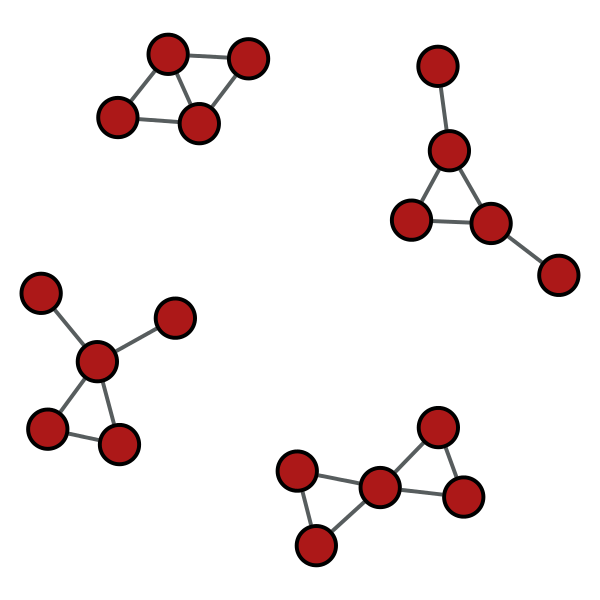
\includegraphics[width=0.4\textwidth]{simple_drawings/combined_subgraphs.png}
  \caption{The named graphs checked for the vertex subgraphs invariant. Clockwise from top: the open-bowtie, bowtie, bull and diamond graph.}
  \label{fig:namedgraphs}
\end{figure}

\section{Submitted sequences}
\label{app:submittedseq}

Primary sequences are those involving a single invariant, while secondary sequences are those that involve the union of two invariants.
The sequences already present in the OEIS served as a useful check on the accuracy of our programs.

\newcommand{\VARsubgraphfree}[1]{g)}

\begin{longtable}{ l l}
\toprule
Invariant symbol & Description \\
\midrule
$\VARautomorphismgroupn$ & Automorphism group size \\
$\VARchromaticnumber$ & Chromatic number \\
$\VARedgeconnectivity$, $\VARedgeconnectivity$ & Vertex/Edge connectivity \\
$\VARdiameter$ & diameter \\
$\VARgirth$ & girth \\
$\VARnarticulationpoints$ & number of articulation points \\
\end{longtable}

\subsection{Primary sequences}

\begin{longtable}{ l l r r r r r r r r r r}
\toprule
OEIS & Invariant & \multicolumn{10}{l}{Sequence} \\
\midrule\bottomrule
\OEIS{A241454} & $\VARautomorphismgroupn =2$ & 0 & 1 & 1 & 2 & 9 & 37 & 317 & 4098 & 84602 & 2933996 \\
\OEIS{A241455} & $\VARautomorphismgroupn =4$ & 0 & 0 & 0 & 1 & 3 & 28 & 198 & 1971 & 29047 & 672516 \\
\OEIS{A241456} & $\VARautomorphismgroupn =6$ & 0 & 0 & 1 & 1 & 1 & 7 & 31 & 221 & 3025 & 68033 \\
\OEIS{A241457} & $\VARautomorphismgroupn =8$ & 0 & 0 & 0 & 1 & 2 & 9 & 55 & 499 & 6017 & 107312 \\
\OEIS{A241458} & $\VARautomorphismgroupn =10$ & 0 & 0 & 0 & 0 & 1 & 1 & 1 & 3 & 13 & 123 \\
\OEIS{A241459} & $\VARautomorphismgroupn =12$ & 0 & 0 & 0 & 0 & 3 & 10 & 51 & 356 & 3395 & 49862 \\
\OEIS{A241460} & $\VARautomorphismgroupn =14$ & 0 & 0 & 0 & 0 & 0 & 0 & 2 & 2 & 2 & 6 \\
\OEIS{A241461} & $\VARautomorphismgroupn =16$ & 0 & 0 & 0 & 0 & 0 & 3 & 10 & 123 & 992 & 14026 \\
\OEIS{A241462} & $\VARautomorphismgroupn =20$ & 0 & 0 & 0 & 0 & 0 & 0 & 2 & 6 & 29 & 199 \\
\OEIS{A241463} & $\VARautomorphismgroupn =24$ & 0 & 0 & 0 & 1 & 1 & 1 & 14 & 118 & 1247 & 17191 \\
\OEIS{A241464} & $\VARautomorphismgroupn =36$ & 0 & 0 & 0 & 0 & 0 & 1 & 3 & 16 & 132 & 1341 \\
\OEIS{A241465} & $\VARautomorphismgroupn =48$ & 0 & 0 & 0 & 0 & 0 & 4 & 14 & 65 & 504 & 5215 \\
\OEIS{A241466} & $\VARautomorphismgroupn =72$ & 0 & 0 & 0 & 0 & 0 & 1 & 2 & 16 & 124 & 1070 \\
\OEIS{A241467} & $\VARautomorphismgroupn =120$ & 0 & 0 & 0 & 0 & 1 & 1 & 1 & 5 & 21 & 211 \\
\OEIS{A241468} & $\VARautomorphismgroupn =144$ & 0 & 0 & 0 & 0 & 0 & 0 & 3 & 12 & 51 & 477 \\
\OEIS{A241469} & $\VARautomorphismgroupn =240$ & 0 & 0 & 0 & 0 & 0 & 0 & 3 & 8 & 51 & 336 \\
\OEIS{A241470} & $\VARautomorphismgroupn =720$ & 0 & 0 & 0 & 0 & 0 & 1 & 1 & 4 & 13 & 60 \\
\OEIS{A241471} & $\VARautomorphismgroupn =5040$ & 0 & 0 & 0 & 0 & 0 & 0 & 1 & 1 & 1 & 5 \\
\OEIS{A241702} & $\VARchromaticnumber =7$ & 0 & 0 & 0 & 0 & 0 & 0 & 1 & 6 & 110 & 4125 \\
\OEIS{A241703} & $\VARedgeconnectivity =4$ & 0 & 0 & 0 & 0 & 1 & 3 & 25 & 378 & 14306 & 1141575 \\
\OEIS{A241704} & $\VARedgeconnectivity =5$ & 0 & 0 & 0 & 0 & 0 & 1 & 3 & 41 & 1095 & 104829 \\
\OEIS{A241705} & $\VARedgeconnectivity =6$ & 0 & 0 & 0 & 0 & 0 & 0 & 1 & 4 & 65 & 3441 \\
\OEIS{A241706} & $\VARdiameter =2$ & 0 & 0 & 1 & 4 & 14 & 59 & 373 & 4154 & 91518 & 4116896 \\
\OEIS{A241707} & $\VARdiameter =3$ & 0 & 0 & 0 & 1 & 5 & 43 & 387 & 5797 & 148229 & 6959721 \\
\OEIS{A241708} & $\VARdiameter =4$ & 0 & 0 & 0 & 0 & 1 & 8 & 82 & 1027 & 19320 & 598913 \\
\OEIS{A241709} & $\VARdiameter =5$ & 0 & 0 & 0 & 0 & 0 & 1 & 9 & 125 & 1818 & 37856 \\
\OEIS{A241710} & $\VARdiameter =6$ & 0 & 0 & 0 & 0 & 0 & 0 & 1 & 12 & 180 & 2928 \\
\OEIS{A241711} & $\VARgirth =3$ & 0 & 0 & 1 & 3 & 15 & 93 & 792 & 10833 & 259420 & 11704309 \\
\OEIS{A241712} & $\VARgirth =4$ & 0 & 0 & 0 & 1 & 2 & 11 & 43 & 234 & 1498 & 11451 \\
\OEIS{A241713} & $\VARgirth =5$ & 0 & 0 & 0 & 0 & 1 & 1 & 5 & 18 & 82 & 539 \\
\OEIS{A241714} & $\VARgirth =6$ & 0 & 0 & 0 & 0 & 0 & 1 & 1 & 7 & 25 & 137 \\
\OEIS{A241715} & $\VARgirth =7$ & 0 & 0 & 0 & 0 & 0 & 0 & 1 & 1 & 6 & 20 \\
\OEIS{A241767} & $\VARnarticulationpoints =1$ & 0 & 0 & 1 & 2 & 7 & 33 & 244 & 2792 & 52448 & 1690206 \\
\OEIS{A241768} & $\VARnarticulationpoints =2$ & 0 & 0 & 0 & 1 & 3 & 17 & 101 & 890 & 11468 & 239728 \\
\OEIS{A241769} & $\VARnarticulationpoints =3$ & 0 & 0 & 0 & 0 & 1 & 5 & 32 & 242 & 2461 & 35839 \\
\OEIS{A241770} & $\VARnarticulationpoints =4$ & 0 & 0 & 0 & 0 & 0 & 1 & 7 & 60 & 527 & 6056 \\
\OEIS{A241771} & $\VARnarticulationpoints =5$ & 0 & 0 & 0 & 0 & 0 & 0 & 1 & 9 & 97 & 1029 \\

\OEIS{A241782} & $\VARissubgraphfreeKfive =0$ & 1 & 1 & 2 & 6 & 20 & 107 & 802 & 10252 & 232850 & 9905775 \\
\OEIS{A241784} & $\VARissubgraphfreeCfive =0$ & 1 & 1 & 2 & 6 & 13 & 44 & 144 & 577 & 2457 & 12499 \\
\OEIS{A242790} & $\VARissubgraphfreediamond =0$ & 1 & 1 & 2 & 4 & 11 & 39 & 165 & 967 & 7684 & 87012 \\
\OEIS{A242792} & $\VARissubgraphfreebowtie =0$ & 1 & 1 & 2 & 6 & 15 & 60 & 273 & 1769 & 14836 & 174111 \\
\OEIS{A242791} & $\VARissubgraphfreeopenbowtie =0$ & 1 & 1 & 2 & 6 & 11 & 34 & 98 & 408 & 1957 & 12740 \\

\OEIS{A243243} & $\VARissubgraphfreeCfour >0$ & 0 & 0 & 0 & 3 & 13 & 93 & 796 & 10931 & 260340 & 11713182 \\
\OEIS{A243246} & $\VARissubgraphfreeCfive >0$ & 0 & 0 & 0 & 0 & 8 & 68 & 709 & 10540 & 258623 & 11704072 \\
\OEIS{A243245} & $\VARissubgraphfreeKthree >0$ & 0 & 0 & 1 & 3 & 15 & 93 & 794 & 10850 & 259700 & 11706739 \\
\OEIS{A243244} & $\VARissubgraphfreeKfour >0$ & 0 & 0 & 0 & 1 & 4 & 30 & 317 & 5511 & 165165 & 8932499 \\
\OEIS{A243242} & $\VARissubgraphfreeKfive >0$ & 0 & 0 & 0 & 0 & 1 & 5 & 51 & 865 & 28230 & 1810796 \\
\OEIS{A243250} & $\VARissubgraphfreediamond >0$ & 0 & 0 & 0 & 2 & 10 & 73 & 688 & 10150 & 253396 & 11629559 \\
\OEIS{A243248} & $\VARissubgraphfreebull >0$ & 0 & 0 & 0 & 0 & 12 & 86 & 773 & 10777 & 259390 & 11705139 \\
\OEIS{A243249} & $\VARissubgraphfreebowtie >0$ & 0 & 0 & 0 & 0 & 6 & 52 & 580 & 9348 & 246244 & 11542460 \\
\OEIS{A243247} & $\VARissubgraphfreeopenbowtie >0$ & 0 & 0 & 0 & 0 & 10 & 78 & 755 & 10709 & 259123 & 11703831 \\

\OEIS{A241814} & $\VARisdistanceregular =1$ & 1 & 1 & 1 & 2 & 2 & 4 & 2 & 5 & 4 & 7 \\
\OEIS{A241839} & $\VARiskregular =0$ & 1 & 0 & 1 & 4 & 19 & 107 & 849 & 11100 & 261058 & 11716404 \\
\OEIS{A241840} & $\VARisdistanceregular =0$ & 0 & 0 & 1 & 4 & 19 & 108 & 851 & 11112 & 261076 & 11716564 \\
\OEIS{A241841} & $\VARistree =0$ & 0 & 0 & 1 & 4 & 18 & 106 & 842 & 11094 & 261033 & 11716465 \\
\OEIS{A241842} & $\VARisintegral =0$ & 0 & 0 & 1 & 4 & 18 & 106 & 846 & 11095 & 261056 & 11716488 \\
\OEIS{A241843} & $\VARischordal =0$ & 0 & 0 & 0 & 1 & 6 & 54 & 581 & 9503 & 249169 & 11607032 \\
\OEIS{A242952} & $\VARisrealspectrum =1$ & 1 & 1 & 1 & 3 & 11 & 54 & 539 & 7319 & 209471 & 10000304 \\
\OEIS{A242953} & $\VARisrealspectrum =0$ & 0 & 0 & 1 & 3 & 10 & 58 & 314 & 3798 & 51609 & 1716267 \\
\OEIS{A243241} & $\VARisstronglyregular =0$ & 0 & 0 & 1 & 4 & 19 & 109 & 852 & 11114 & 261077 & 11716566 \\

%\OEIS{A243251} & $\VARhasfractionaldualitygapvertexchromatic =1$ & 0 & 0 & 0 & 0 & 1 & 3 & 33 & 496 & 16464 & 969293 \\
%\OEIS{A243252} & $\VARhasfractionaldualitygapvertexchromatic =0$ & 1 & 1 & 2 & 6 & 20 & 109 & 820 & 10621 & 244616 & 10747278 \\
%\OEIS{A243781} & $\VARmaximalindependentvertexset =2$ & 0 & 0 & 1 & 4 & 11 & 34 & 103 & 405 & 1892 & 12166 \\
%\OEIS{A243782} & $\VARmaximalindependentvertexset =3$ & 0 & 0 & 0 & 1 & 8 & 63 & 524 & 5863 & 100702 & 2880002 \\
%\OEIS{A243783} & $\VARmaximalindependentvertexset =4$ & 0 & 0 & 0 & 0 & 1 & 13 & 205 & 4308 & 135563 & 7161399 \\
%\OEIS{A243784} & $\VARmaximalindependentvertexset =5$ & 0 & 0 & 0 & 0 & 0 & 1 & 19 & 513 & 21782 & 1576634 \\

\end{longtable}

\subsection{Secondary sequences}
\note{Add table of secondary sequences}

\section{Relations}
\label{app:relations}
\note{Add table of secondary sequences}

\end{appendices}

\end{document}
